Harry Roberts, a naturalist from the Alaska fish and Game department, studies grizzly
bears with the goal of maintaining a healthy population. Measurements on $n=61$ bears
provided the following summary statistics (see also Exercise 8.23):

\begin{center}
    \begin{tabular}{p{5em} | p{1cm} p{1cm} p{1cm} p{1cm} p{1cm} p{1cm}}
        Variable & Weight (kg) & Body length (cm) & Neck (cm) & Girth (cm) & Head length (cm) & Head width (cm) \\
        \hline
        \multicolumn{1}{m{5em}|}{Sample mean $\bar{x}$} &
        \multicolumn{1}{m{1cm}}{95.52} &
        \multicolumn{1}{m{1cm}}{164.38} &
        \multicolumn{1}{m{1cm}}{55.69} &
        \multicolumn{1}{m{1cm}}{93.39} &
        \multicolumn{1}{m{1cm}}{17.98} &
        \multicolumn{1}{m{1cm}}{31.13}
    \end{tabular}
\end{center}

Covariance matrix

\[
    \textbf{S}
    =
    \begin{bNiceArray}{rrrrrr}
        3266.46 & 1343.97 & 731.54 & 1175.50 & 162.68 & 238.37 \\
        1343.97 & 721.91  & 324.25 & 537.35  & 80.17  & 117.73 \\
        731.54  & 324.25  & 179.28 & 281.17  & 39.15  & 56.80  \\
        1175.50 & 537.35  & 281.17 & 474.98  & 63.73  & 94.85  \\
        162.68  & 80.17   & 39.15  & 63.73   & 9.95   & 13.88  \\
        238.37  & 117.73  & 56.80  & 94.85   & 13.88  & 21.26
    \end{bNiceArray}
\]

\begin{enumerate}[label=(\alph*)]
    \item Obtain the large sample 95\% simultaneous confidence intervals for the six population mean body measurements.
    \newline
    \par
    From page 235 I used:
    \[
        \bar{x}_{i} \pm \sqrt{\chi_{p}^{2}(\alpha)} \sqrt{\frac{S_{ii}}{n}}
    \]
    where $\chi_{6}^{2}(0.05) = 12.59$
    \[
    \begin{NiceArray}{rrrr}
       95.52 \pm \sqrt{12.59} \frac{\sqrt{3266.46}}{\sqrt{61}} & \text{contains }\mu_{1} & \text{ or } & 69.55 \leq \mu_{1} \leq 121.49 \\
       164.38 \pm \sqrt{12.59} \frac{\sqrt{721.91}}{\sqrt{61}} & \text{contains }\mu_{2} & \text{ or } & 152.17 \leq \mu_{2} \leq 176.59 \\
       55.69 \pm \sqrt{12.59} \frac{\sqrt{179.28}}{\sqrt{61}} & \text{contains }\mu_{3} & \text{ or } & 49.61 \leq \mu_{3} \leq 61.77  \\
       93.39 \pm \sqrt{12.59} \frac{\sqrt{474.98}}{\sqrt{61}} & \text{contains }\mu_{4} & \text{ or } & 83.49 \leq \mu_{4} \leq 103.29 \\
       17.98 \pm \sqrt{12.59} \frac{\sqrt{9.95}}{\sqrt{61}} & \text{contains }\mu_{5} & \text{ or } & 16.55 \leq \mu_{5} \leq 19.41  \\
       31.13 \pm \sqrt{12.59} \frac{\sqrt{21.26}}{\sqrt{61}} & \text{contains }\mu_{6} & \text{ or } & 29.04 \leq \mu_{6} \leq 33.22
    \end{NiceArray}
    \]
    \item Obtain the large sample 95\% simultaneous confidence ellipse for mean weight and mean girth.
    
    \begin{figure}[H]
        \centering
            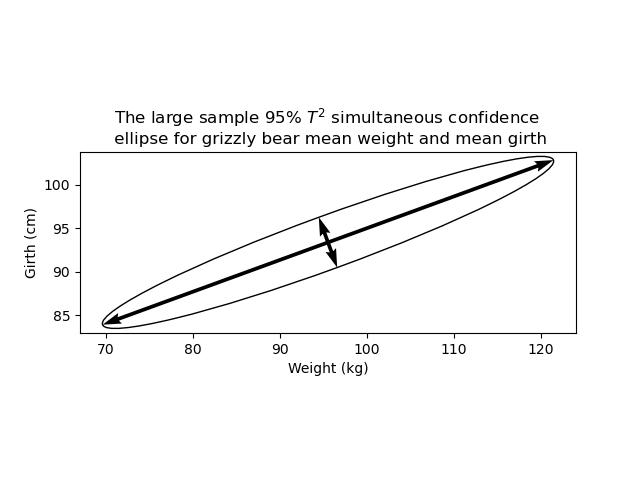
\includegraphics[scale=0.75]{./python/chapter-5/Question-5-9-b.png}
    \end{figure}

    \item Obtain the 95\% Bonferroni confidence intervals for the six means in Part a.
    \newline
    \par
    They didn't explicitly say ``large sample'', but I'm going to assume they mean that. This time, from page 237, I used:
    \[
        \bar{x}_{i} \pm z(\alpha/(2m)) \sqrt{\frac{S_{ii}}{n}}
    \]
    where $z(0.05/12) = 2.64$
    \[
        \begin{NiceArray}{rrrr}
            95.52 \pm 2.64 \frac{\sqrt{3266.46}}{\sqrt{61}} & \text{contains }\mu_{1} & \text{ or } & 76.21 \leq \mu_{1} \leq 114.83 \\
            164.38 \pm 2.64 \frac{\sqrt{721.91}}{\sqrt{61}} & \text{contains }\mu_{2} & \text{ or } & 155.30 \leq \mu_{2} \leq 173.46 \\
            55.69 \pm 2.64 \frac{\sqrt{179.28}}{\sqrt{61}} & \text{contains }\mu_{3} & \text{ or } & 51.17 \leq \mu_{3} \leq 60.21  \\
            93.39 \pm 2.64 \frac{\sqrt{474.98}}{\sqrt{61}} & \text{contains }\mu_{4} & \text{ or } & 86.03 \leq \mu_{4} \leq 100.75 \\
            17.98 \pm 2.64 \frac{\sqrt{9.95}}{\sqrt{61}} & \text{contains }\mu_{5} & \text{ or } & 16.91 \leq \mu_{5} \leq 19.05  \\
            31.13 \pm 2.64 \frac{\sqrt{21.26}}{\sqrt{61}} & \text{contains }\mu_{6} & \text{ or } & 29.57 \leq \mu_{6} \leq 32.69
        \end{NiceArray}
    \]

    \item Refer to Part b. Construct the 95\% Bonferroni confidence rectangle for the mean weight and mean girth using $m = 6$. Compare this rectangle with the confidence ellipse in Part b.
    
    \begin{figure}[H]
        \centering
            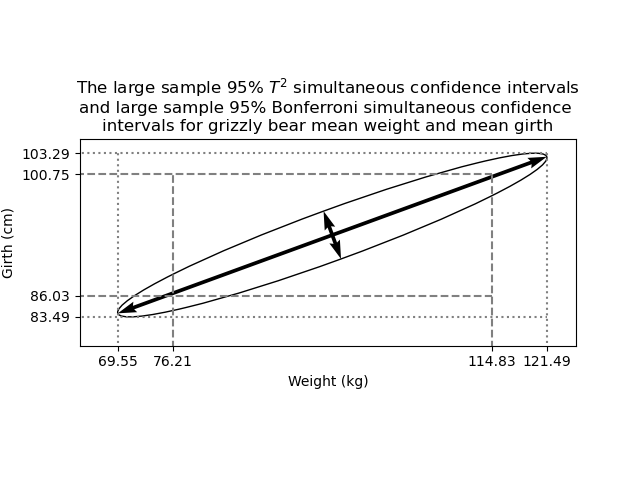
\includegraphics[scale=0.75]{./python/chapter-5/Question-5-9-d.png}
    \end{figure}

    \item Obtain the 95\% Bonferroni confidence interval for
    \[
        \text{mean head width} - \text{mean head length}
    \]
    using $m = 6 + 1 = 7$ to allow for this statement as well as statements about each
    individual mean.

    \[
        \textbf{a}^{\prime}
        =
        \begin{bNiceArray}{rrrrrr}
            0, & 0, & 0, & 0, & -1, & 1
        \end{bNiceArray}
    \]
    using
    \[
        \textbf{a}^{\prime}
        \bar{\textbf{x}}
        \pm
        z\left(\frac{\alpha}{2(m+1)}\right)
        \sqrt{\frac{\textbf{a}^{\prime}\textbf{S}\textbf{a}}{n}}
    \]
    \[
        \textbf{a}^{\prime}
        \bar{\textbf{x}}
        =
        \begin{bNiceArray}{rrrrrr}
            0, & 0, & 0, & 0, & -1, & 1
        \end{bNiceArray}
        \begin{bNiceArray}{c}
            95.52 \\
            164.38 \\
            55.69 \\
            93.39 \\
            17.98 \\
            31.13
        \end{bNiceArray}
        =
        31.13 - 17.98
        =
        13.15
    \]
    \begin{multline*}
        \textbf{a}^{\prime}\textbf{S}\textbf{a}
        =
        \begin{bNiceArray}{rrrrrr}
            0, & 0, & 0, & 0, & -1, & 1
        \end{bNiceArray} \\
        \times
        \begin{bNiceArray}{rrrrrr}
            3266.46 & 1343.97 & 731.54 & 1175.50 & 162.68 & 238.37 \\
            1343.97 & 721.91  & 324.25 & 537.35  & 80.17  & 117.73 \\
            731.54  & 324.25  & 179.28 & 281.17  & 39.15  & 56.80  \\
            1175.50 & 537.35  & 281.17 & 474.98  & 63.73  & 94.85  \\
            162.68  & 80.17   & 39.15  & 63.73   & 9.95   & 13.88  \\
            238.37  & 117.73  & 56.80  & 94.85   & 13.88  & 21.26
        \end{bNiceArray}
        \begin{bNiceArray}{r}
            0 \\ 0 \\ 0 \\ 0 \\ -1 \\ 1
        \end{bNiceArray}
        =
    \end{multline*}
    \[
        =
        \begin{bNiceArray}{rrrrrr}
            0, & 0, & 0, & 0, & -1, & 1
        \end{bNiceArray} \\
        \begin{bNiceArray}{c}
            75.69 \\
            37.56 \\
            17.65 \\
            31.12 \\
            3.93  \\
            7.38
        \end{bNiceArray}
        =
        7.38 - 3.93
        =
        3.45
    \]
    and $z(0.05/14) = 2.69$
    \[
        \textbf{a}^{\prime}
        \bar{\textbf{x}}
        \pm
        z\left(\frac{\alpha}{2(m+1)}\right)
        \sqrt{\frac{\textbf{a}^{\prime}\textbf{S}\textbf{a}}{n}}
        =
        13.15\
        \pm
        2.69
        \sqrt{
            \frac{3.45}{67}
        }
        =
        [12.523, 13.777]
    \]
    or as
    \[
        12.523 \leq \mu_{6} - \mu_{5} \leq 13.777
    \]

\end{enumerate}